\documentclass{article}
\usepackage{cmap}
\usepackage[utf8]{inputenc}
\usepackage[english,ukrainian]{babel}
\usepackage{graphicx}
\usepackage{geometry}
\usepackage{listings}
\usepackage{amsmath}
\usepackage{float}
\geometry{
	a4paper,
	left=20mm,
	right=20mm,
	top=20mm,
	bottom=20mm
}
\lstset{
	language=c++,
	tabsize=4,
	keepspaces,
	showstringspaces=false,
}
\graphicspath{ {./pictures} }
\setlength{\parindent}{4em}

\newcommand\subject{Операційні системи}
\newcommand\lecturer{старший викладач кафедри ПЗ\\Грицай О.Д.}
\newcommand\teacher{старший викладач кафедри ПЗ\\Грицай О.Д.}
\newcommand\mygroup{ПЗ-22}
\newcommand\lab{6}
\newcommand\theme{Багатопоточність в операційній системі Linux. Створення,
	керування та синхронізація потоків}
\newcommand\purpose{Навчитися створювати потоки та керувати ними в операційній
	системі Linux. Ознайомитися з методами синхронізації потоків в операційній
	системі Linux. Навчитися реалізовувати багатопоточний алгоритм розв’язку
	задачі з використанням синхронізації в операційній системі Linux}

\begin{document}
\begin{normalsize}
	\begin{titlepage}
		\thispagestyle{empty}
		\begin{center}
			\textbf{МІНІСТЕРСТВО ОСВІТИ І НАУКИ УКРАЇНИ\\
				НАЦІОНАЛЬНИЙ УНІВЕРСИТЕТ "ЛЬВІВСЬКА ПОЛІТЕХНІКА"}
		\end{center}
		\begin{flushright}
			Інститут \textbf{КНІТ}\\
			Кафедра \textbf{ПЗ}
		\end{flushright}
		\vspace{200pt}
		\begin{center}
			\textbf{ЗВІТ}\\
			\vspace{10pt}
			До лабораторної роботи № \lab\\
			\textbf{На тему}: “\textit{\theme}”\\
			\textbf{З дисципліни}: “\subject”
		\end{center}
		\vspace{112pt}
		\begin{flushright}
			
			\textbf{Лектор}:\\
			\lecturer\\
			\vspace{28pt}
			\textbf{Виконав}:\\
			
			студент групи \mygroup\\
			Коваленко Д.М.\\
			\vspace{28pt}
			\textbf{Прийняла}:\\
			
			\teacher\\
			
			\vspace{28pt}
			«\rule{1cm}{0.15mm}» \rule{1.5cm}{0.15mm} 2022 р.\\
			$\sum$ = \rule{1cm}{0.15mm}……………\\
			
		\end{flushright}
		\vspace{\fill}
		\begin{center}
			\textbf{Львів — 2022}
		\end{center}
	\end{titlepage}
		
	\begin{description}
		\item[Тема.] \theme.
		\item[Мета.] \purpose.
	\end{description}

	\section*{Лабораторне завдання}
	\begin{enumerate}
		\item Реалізувати заданий алгоритм в окремому потоці
		\item Виконати розпаралелення заданого алгоритму на 2, 4, 8, 16 потоків
		\item Реалізувати можливість зміни/встановлення пріоритету потоку (для
		планування потоків) або встановлення відповідності виконання на ядрі
		\item Реалізувати можливість зробити потік від’єднаним
		\item Реалізувати можливість відміни потоку
		\item Реалізувати синхронізацію потоків за допомогою вказаних методів
		(згідно варіанту)
		\item Порівняти час виконання задачі відповідно до кількості потоків і методу
		синхронізації (чи без синхронізації).
		\item Результати виконання роботи оформити у звіт
	\end{enumerate}
	\begin{center}
		2. Обчислити суму елементів заданого масиву (кількість елементів >10000,
		елементи рандомні) (Синхронізація: семафор, спінблокувавння)
	\end{center}

	\section*{Хід роботи}	
	\begin{lstlisting}
#include "task.h"
#include <unistd.h>
#include "QDebug"

using namespace std;

int numCpus = sysconf(_SC_NPROCESSORS_ONLN);

void* thread_task(void* args) {
	pthread_setcancelstate(PTHREAD_CANCEL_ENABLE, 0);
	pthread_setcanceltype(PTHREAD_CANCEL_ASYNCHRONOUS, 0);
	
	ThreadArgs* targs = (ThreadArgs*)args;
	int start = targs->start;
	int end = targs->end;
	int* sum = targs->sum;
	int* arr = targs->arr;
	sem_t* sem = targs->sem;
	pthread_spinlock_t* spin = targs->spin;
	Task* task = (Task*)targs->task;
	
	task->setStatus(Running);
	int value;
	sem_getvalue(sem, &value);
	if (value == 0) {
		task->setStatus(Waiting);
	}
	sem_wait(sem);
	task->setStatus(Running);
	std::srand(static_cast<unsigned int>(std::time(nullptr)));
	for (int i = start; i < end; i++) {
		arr[i] = rand() % 5;
	}
	
	for (int i = start; i < end; i++) {
		pthread_spin_lock(spin);
		*sum += arr[i];
		pthread_spin_unlock(spin);
	}
	sem_post(sem);
	task->setStatus(Done);
	pthread_exit(NULL);
}

Task::Task(int threadCount, int threadIndex, int arrLen, int* sum, int* arr, sem_t* sem, pthread_spinlock_t* spin) {
	pthread_attr_t attr;
	pthread_attr_init(&attr);
	this->attr = attr;
	pthread_attr_setschedpolicy(&this->attr, SCHED_FIFO);
	ThreadArgs* args = new ThreadArgs(threadCount, threadIndex, arrLen, sum, arr, sem, spin, this);
	if (pthread_create(&this->thread, &attr, &thread_task, args)) {
		qDebug() << "pthread_create error!";
		return;
	}
	this->threadIndex = threadIndex;
	this->setAffinity(this->threadIndex % numCpus);
}

void Task::detach() {
	pthread_detach(this->thread);
	if (this->status != Done) this->status = Detached;
}

void Task::cancel() {
	pthread_cancel(this->thread);
	if (this->status != Done) this->status = Canceled;
}

void Task::setPriority(int n) {
	int policy;
	struct sched_param param;
	
	pthread_getschedparam(this->thread, &policy, &param);
	param.sched_priority = n;
	pthread_setschedparam(this->thread, policy, &param);
}

int Task::getPriority() {
	int policy;
	struct sched_param param;
	pthread_getschedparam(this->thread, &policy, &param);
	return param.sched_priority;
}

void Task::setAffinity(int cpu) {
	cpu_set_t cpuset;
	CPU_ZERO(&cpuset);
	CPU_SET(cpu, &cpuset);
	if (pthread_setaffinity_np(this->thread, sizeof(cpuset), &cpuset)) {
		qDebug() << "pthread_setaffinity_np() error";
	}
}

int Task::getAffinity() {
	cpu_set_t cpuset;
	CPU_ZERO(&cpuset);
	if (pthread_getaffinity_np(this->thread, sizeof(cpuset), &cpuset)) {
		qDebug() << "pthread_attr_getaffinity_np() error";
	}
	for (int i = 0; i < numCpus; i++) {
		if (CPU_ISSET(i, &cpuset)) return i;
	}
	return -1;
}

	\end{lstlisting}
	
	\begin{figure}[H]
		\centering
		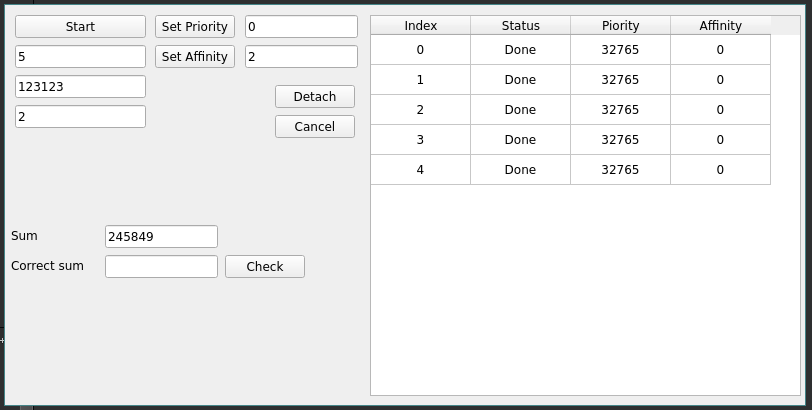
\includegraphics[scale=0.6]{v}
		\caption{Виконання програми}
	\end{figure}
	
	\section*{Висновок}
	Під час виконання лабораторної роботи я навчився створювати потоки та керувати ними в операційній системі Linux. Ознайомився з методами синхронізації потоків в операційній системі Linux. Навчився реалізовувати багатопоточний алгоритм розв’язку
	задачі з використанням синхронізації в операційній системі Linux
	
	 
\end{normalsize}
\end{document}
